\chapter{Adele, Idele und Verallgemeinerte Idealklassengruppen}
\section{Eingeschränkte Produkte}
\Bem{}
Ab sofort heißt ein topologischer Raum \textit{kompakt}, falls er \textit{quasikompakt} und \textit{hausdorffsch} ist.\\
Ein Raum heißt ferner ab jetzt \textit{lokal kompakt}, falls er \textit{hausdorffsch} und \textit{lokal quasikompakt} ist.

\Def{Eingeschränkte Produkte}
Sei $I$ eine Indexmenge, $(G_i)_{i\in I}$ eine Familie lokal kompakter, abelscher Gruppen und $(U_i)_{i\in I}$ eine Familie offener Untergruppen, sodass fast alle $U_i$ zusätzlich kompakt sind.\\
Definiere das \df{restringierte Produkt} bzw. \df{eingeschränkte Produkt} von $(G_i)_i$ bzgl. $(U_i)_i$ durch
\[ \prod_{i\in I}'G_i := \set{(x_i)_i \in \prod_{i\in I}G_i}{ x_i \in U_i \text{ ffa } i \in I } \]
Definiere für eine endliche Menge $J \subset I$
\[ G_J := \prod_{i \in J}G_i \times \prod_{i \in I\setminus J} G_i \]
Dann gilt
\[ \prod_{i\in I}'G_i = \bigcup_{J \text{ endlich}}G_J  \]
Jedes $G_J$ trägt die Produkttopologie und ist lokal kompakt; das restringierte Produkt $\prod_{i\in I}'G_i$ wird nun mit der dadurch induzierten Kolimestopologie versehen. Dadurch ist $\prod_{i\in I}'G_i$ ebenfalls lokal kompakt und für jedes $V \subset \prod_{i\in I}'G_i$ gilt insbesondere
\[ V \subset_o G \Gdw{} V\cap G_J \subset_o G_J \text{ für alle }J \text{ endlich} \]
Die Menge
\[ \set{ \prod_{i \in J}O_i \times \prod_{i \in I\setminus J}U_i }{J \subset I \text{ endlich und } 1 \in O_i \subset_o G_i} \]
bildet eine Umgebungsbasis der Eins in $\prod_{i\in I}'G_i$.\\
Ferner wird folgende universelle Abbildungseigenschaft für jede hausdorffsche, abelsche Gruppe $Z$ erfüllt
\[ \Hom{cts}{\prod_{i\in I}'G_i}{Z} = \set{(f_i)_i \in \prod_{i \in I} \Hom{cts}{G_i}{Z} }{ \text{ffa } i \in I \text{ ist } f_i(U_i) \text{ in jedem }1 \in U\subset_o Z \text{ enthalten} } \]


\section{Adele und Idele}
\Def{Adelering und Idelering}
Sei $K$ ein globaler Körper, $S$ die Menge aller Stellen von $K$. Definiere den \df{Adelering} von $K$ durch das restringierte Produkt
\[ \A_K := \prod'_{v\in S} K_v \text{ bzgl. } (\O_v)_{v\in S} \]
und die \df{Idelegruppe} durch
\[ \A_K^\times := \prod'_{v\in S}K_v^\times \text{ bzgl. } (\O_v^\times)_{v\in S} \]

\Bem{}
\[(\A_K)^\times = \A_K^\times \]
\Def{Hauptadele und Hauptidele}
Es liegen folgende Homomorphismen vor
\begin{align*}
K & \Inj{} \A_K && K^\times \Inj{} \A_K^\times\\
a & \longmapsto (a)_v && a\longmapsto (a)_v
\end{align*}
Die Bilder dieser Inklusionen nennen wir \df{Hauptadele} bzw. \df{Hauptidele}.\\
Die \df{Idele-Klassengruppe} ist definiert durch
\[ C_K := \A_K^\times / K^\times \]
Ferner liegt folgender stetiger multiplikativer Monoid-Homomorphismus vor
\begin{align*}
\bet{\cdot} : \A_K &\Pfeil{} \R_{\geq 0}\\
(a_v)_v & \longmapsto \bet{a} := \prod_{v}\bet{a_v}_v
\end{align*}

\Satz{Produktformel}
Sei $K$ global, dann gilt für alle $a \in K^\times$
\[ \bet{a} = 1 \]

\Satz{}
Sei $K$ global.
\begin{itemize}
\item $K$ liegt in $\A_K$ diskret und $\A_K/K$ ist kompakt.
\item Definiere
\[ \A_K^1 := \set{a\in\A_K^\times}{ \bet{a} = 1 } \]
$K^\times$ liegt in $\A_K^1$ diskret und $C^1_K:= \A_K^1/K^\times$ ist kompakt.
\end{itemize}

\Bem{}
$C_K = \A_K^\times/K^\times$ ist im Allgemeinem nicht kompakt.

\Bem{Idealklassengruppe}
Sei $K$ ein Zahlkörper, $\I$ bezeichne die Menge der gebrochenen Ideale von $K$, $\P$ die Menge der gebrochenen Hauptideale.\\
Die \df{Idealklassengruppe} ist definiert durch
\[Cl_K = \I/\P \]
Bezeichnet $S_f$ die Menge der endlichen Stellen von $K$ und $S_\infty$ die Menge der unendlichen Stellen von $K$, so definiere
\[ \U := \prod_{v\in S_\infty}K_v^\times \times \prod_{v\in S_f} \O_v^\times \subset \A_K^\times \]
Es gilt
\[ \A_K^\times / \U \isom{} \bigoplus_{v\in S_f} K_v^\times / \O_v^\times \isom{} \I  \]
Definiert man ferner $\overline{\U} := K^\times\cdot\U/K^\times$, so gilt
\[ C_K / \overline{\U} \isom{} \A_K^\times / K^\times \U = \I / \P \isom{} Cl_K \]

\Def{Verallgemeinerte Idealklassengruppe}
Sei $K$ ein Zahlkörper.\\
Definiere für ein Ideal $0\neq \af \subset \O_K$
\[ \U(\af) := \prod_{v\in S}U_v(\af) \subset \U \]
wobei
\[ U_v(\af) := \left\lbrace
\begin{aligned}
\{x \in \O_{K_v}~|~x \equiv 1 \mod{\af\O_{K_v}}\} = 1 + \mf_v^{n_v(\af)} = 1 + \af \O_{K_v} && v \in S_f\\
K_v^\times && v \text{ komplex}\\
\R_{>0} \cap K^\times_v && v \text{ reell}
\end{aligned}
\right. \]
Die \df{verallgemeinerte Idealklassengruppe} ist definiert durch
\[Cl(K, \af) = C_K / \overline{\U(\af)} \]
Es gilt für Ideale $\af,\bf$
\[ \af \leq \bf \Gdw{} \U(\af) \leq \U(\bf) \Gdw{} Cl(K,\af) \surj{} Cl(K,\bf) \]
und
\[ Cl(K,\O_K) = Cl_K \]

\Bem{Alternative Beschreibung der Idealklassengruppe}
Sei $K$ ein Zahlkörper, $0\neq \af \subset \O_K$ ein Ideal.\\
Es sei
\[ S(\af) := \set{v \in S_f}{n_v(\af) \neq 0} \]
Definiere für ein Ideal $0\neq \af \subset \O_K$ die Gruppe der zu $\af$ teilerfremden gebrochenen Ideale
\[ \I(\af) := \set{\bf\i \cf}{\bf,\cf \trianglelefteq \O_K \text{ teilerfremd zu } \af} \isom{} \bigoplus_{v\in S_f \setminus S(\af)}\Z \]
und die Gruppe der $\af$ teilerfremden gebrochenen Hauptideale
\[ \P(\af) := \set{(\alpha) \in K^\times}{\alpha \text{ ist lokal positiv und }\forall v \in S(\af): \alpha \in 1 + \af\O_{K_v}}  \]

\Bem{}
Im Allgemeinem gilt
\[ \P(\af) \subsetneq \P \cap \I(\af) \]
In jedem Fall gilt wegen dem Approximationsatz
\[ \I(\af) / \P \cap \I(\af) = \I / \P = Cl(K) \]

\Satz{}
Sei $K$ ein Zahlkörper, $0\neq \af \subset \O_K$ ein Ideal.\\
Setze
\[ S:= S_\infty \cup S(\af) \]
Beachte, dass $U_v(\af) = \O_{K_v}^\times$ für $v \notin S$ gilt. Wir erklären folgenden Homomorphismus
\begin{align*}
\phi : \I(\af) \isom{} \bigoplus_{v\notin S} \Z \isom{} \bigoplus_{v\notin S} K_v^\times / U_v(\af) \subset \A_K^\times / \U(\af) \surj{} C_K / \overline{\U(\af)} = Cl(K,\af)  
\end{align*}
Es gilt
\begin{itemize}
\item $\phi$ induziert einen Isomorphismus
\[ \phi : \I(\af) / \P(\af) \Pfeil{} Cl(K,\af) \]
\item Es liegt folgende kurze exakte Sequenz vor
\[ 1 \Pfeil{} \klam{ \bigoplus_{v \text{ reell}} \R^\times / \R_{>0} \oplus (\O_K / \af)^\times } / \O_K^\times \Pfeil{} Cl(K,\af) \Pfeil{} Cl(K) \Pfeil{} 1 \]
Insbesondere ist $Cl(K,\af)$ endlich.
\end{itemize}

\Satz{Approximationssatz}
Sei $K$ ein Zahlkörper, $S$ eine endliche Stellenmenge. Für jedes $v \in S$ sei ein $x_v \in K$ vorgegeben. Dann existiert für jedes $\epsilon >0$ ein $x \in K$, sodass für alle $v \in S$ gilt
\[ \bet{x-x_v}_v < \epsilon \]

\Def{}
Sei $K$ ein Zahlkörper, $0\neq \af \subset \O_K$ ein Ideal, $S = S_\infty \cup S(\af)$.\\
Definiere
\[ K_\af^\times := \Ker\klam{ K^\times \pfeil{} \bigoplus_{v\in S } K_v^\times / U_v(\af)}  \]
und
\[\O_{K,\af}^\times := K_\af^\times \cap \O_K^\times \]
Dann liegt folgende Isomorphie vor
\[ K_\af^\times / \O_{K,\af}^\times = \P(\af) \]

\Lem{}
Folgende Sequenz ist exakt
\[ 1 \Pfeil{} K_\af^\times \Pfeil{} K^\times \Pfeil{} \bigoplus_{v\in S} K_v^\times/U_v(\af) \Pfeil{} 1 \]

\Satz{Schlangenlemma}
Sei folgendes kommutative Diagramm von $R$-Moduln gegeben
\begin{center}
\begin{tikzpicture}[scale =2]
\node (O1) at (-1,0)  {$0$};
\node (A1) at (0,1)  {$A$};
\node (A2) at (0,0)  {$A'$};
\node (B1) at (1,1)  {$B$};
\node (B2) at (1,0)  {$B'$};
\node (C1) at (2,1)  {$C$};
\node (C2) at (2,0)  {$C'$};
\node (O2) at (3,1)  {$0$};

\draw[->] (O1) -> (A2);
\draw[->] (A2) -> (B2);
\draw[->] (B2) -> (C2);

\draw[->] (A1) -> (B1);
\draw[->] (B1) -> (C1);
\draw[->] (C1) -> (O2);

\draw[->] (A1) -> (A2) node[midway, left]{$a$};
\draw[->] (B1) -> (B2) node[midway, left]{$b$};
\draw[->] (C1) -> (C2) node[midway, left]{$c$};
\end{tikzpicture}
\end{center}
Es liegt folgende exakte Sequenz vor
\[ \Ker a \Pfeil{} \Ker b \Pfeil{} \Ker c \Pfeil{\delta} \Coker a \Pfeil{} \Coker b \Pfeil{} \Coker c \]

\Bem{}
Definiere
\[ \A_{K,\af}^\times := \prod_{v \in S}U_v(\af) \times \prod'_{v\notin S} K_v^\times \]
dann liegt folgende Isomorphie vor
\[ \A_{K,\af}^\times / K_\af^\times \Pfeil{\isom{}} \A_K^\times / K^\times \]
und folgende surjektive Abbildung
\begin{align*}
\Psi_\af : \A_{K,\af}^\times &\Pfeil{} \I(\af)\\
(a)_v & \longmapsto (a) := \prod_{v\in S_f}\pf_v^{v(a_v)}
\end{align*}


\section{Normgruppen}
\Def{Spur und Norm}
Sei $L|K$ eine endliche, galoissche Erweiterung globaler Körper.\\
Definiere die \df{Spurabbildung} auf den Adelen durch
\begin{align*}
Tr_{L|K} : \A_L & \Pfeil{} \A_K\\
(x_w)_w & \longmapsto \klam{\sum_{w |v}Tr_{L_w|K_v}(x_w) }_v
\end{align*}
und die \df{Normabbildung} durch
\begin{align*}
N_{L|K} : \A_L^\times & \Pfeil{} \A_K^\times\\
(x_w)_w & \longmapsto \klam{\prod_{w |v}N_{L_w|K_v}(x_w) }_v
\end{align*}
$G(L|K)$ operiert auf den Adelen bzw. Idelen durch
\[ \klam{(x_w)_w}^\sigma := (x_w^\sigma)_{w^\sigma} = (x_{w^{\sigma\i}}^\sigma)_w \]
für $(x_w)_w \in \A_L$. Es gilt ferner
\[ \A_L^{G(L|K)} = \A_K \text{ und } (\A_L^\times)^{G(L|K)} = \A_K^\times \]

\Bem{}
Es bezeichne $G = G(L|K)$. Da $L^\times \inj{} \A_L^\times$ eine Inklusion von $G$-Moduln ist, ist auch $C_L = \A_L^\times / L^\times$ ein $G$-Modul.\\
Da die erste Kohomologiegruppe $H^1(G,L^\times) = 1$ verschwindet laut Hilbert '90, ist der Invariantenfunktor
\begin{align*}
G-\Mod & \Pfeil{} \textbf{Ab}\\
M & \longmapsto M^G := \{m \in M ~|~ \forall g \in G: m^g = m\}
\end{align*}
exakt, ergo ergibt sich folgendes kommutative Diagramm
\begin{center}
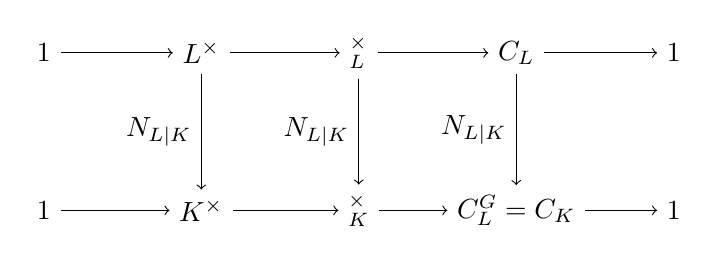
\begin{tikzpicture}[scale =2]
\node (O1) at (-1,0)  {$1$};
\node (O4) at (3,0)  {$1$};
\node (A1) at (0,1)  {$L^\times$};
\node (A2) at (0,0)  {$K^\times$};
\node (B1) at (1,1)  {$\A_L^\times$};
\node (B2) at (1,0)  {$\A_K^\times$};
\node (C1) at (2,1)  {$C_L$};
\node (C2) at (2,0)  {$C_L^G = C_K$};
\node (O2) at (3,1)  {$1$};
\node (O3) at (-1,1)  {$1$};

\draw[->] (O1) -> (A2);
\draw[->] (A2) -> (B2);
\draw[->] (B2) -> (C2);
\draw[->] (C2) -> (O4);

\draw[->] (O3) -> (A1);
\draw[->] (A1) -> (B1);
\draw[->] (B1) -> (C1);
\draw[->] (C1) -> (O2);

\draw[->] (A1) -> (A2) node[midway, left]{$N_{L|K}$};
\draw[->] (B1) -> (B2) node[midway, left]{$N_{L|K}$};
\draw[->] (C1) -> (C2) node[midway, left]{$N_{L|K}$};
\end{tikzpicture}
\end{center}
Es folgt nun
\begin{itemize}
\item $N_{L|K}C_L = K^\times N_{L|K}\A_L^\times ~/~ K^\times$
\item $C_K / N_{L|K}C_L = \A_K^\times ~/~ (K^\times  N_{L|K}\A_L^\times)$
\end{itemize}

\Def{Zulässige Ideale}
Sei $K$ ein Zahlkörper. Ein Ideal $0\neq \af \subset \O_K$ heißt \df{zulässig} für eine endliche, galoissche Erweiterung $L|K$, falls für alle Stellen $v$ von $K$ und allen $w$ über $v$ gilt
\[ U_v(\af) \subseteq N_{L_w|K_v}L_w^\times \]
\paragraph{Bemerkung} Für unendliche Stellen ist diese Bedingung immer erfüllt.\\
Für endliche, unverzweigte Stellen ist diese Bedingung ebenfalls immer erfüllt.\\
Bezeichnet $S$ die Menge aller Stellen, die in $L$ verzweigen, so wähle $\af$ dergestalt, dass für alle $v \in S$ und $w$ über $v$ gilt
\[ [L_w : K_v] ~|~ v(\af) \]
Es gilt in diesem Fall
\[ U_v(\af) = 1+\af \O_{K_v} = 1 + \mf_v^{v(\af)} \subset (K^\times_v)^{v(\af)}  \subset (K^\times_v)^{[L_w:K_v]} = N_{L_w|K_v}K^\times_v \subset N_{L_w|K_v}L_w^\times  \]
Bezüglich Teilbarkeit existiert für $L|K$ ferner stets ein kleinstes zulässiges Ideal $\ff$.

\Satz{}
\begin{itemize}
\item Ist $L|K$ eine endliche, unverzweigte Erweiterung lokaler Körper, so ist folgende Norm
\[ N_{L|K} : \O_L^\times \Pfeil{} \O_K^\times \]
surjektiv.
\item Sei $L|K$ eine endliche, galoissche Erweiterung globaler Körper, $\af$ ein zulässiges Ideal und $\ff$ das kleinste zulässige Ideal für $L|K$.\\
Definiere die Menge der gebrochenen Ideale in $L$ mit zu $\af$ teilerfremden Träger durch
\[ \I_L(\af) := \set{\bf \in \I_L}{ \Pf | \bf \impl{} \Pf \nmid \af\O_L } \]
und
\[ \Nc(\af) := N_{L|K}\I_L(\af) = \set{N_{L|K}\bf}{\bf \in \I_L(\af)} \subset \I(\af) \]
Die Inklusion
\[ \I(\af) \Inj{} \I(\ff) \]
induziert einen Isomorphismus
\[ \I(\af) / (\P(\af) \Nc(\af)) \isom{} \I(\ff) / (\P(\ff) \Nc(\ff)) \]
Insbesondere gilt
\[ \P(\ff) \Nc(\ff) \cap \I(\af) = \P(\af)\Nc(\af) \]
Stimmen die \df{Träger} von $\ff$ und $\af$ überein, d.\,h.
\[ \textsf{supp}(\af) := \set{\pf \in \textsf{Spec}\O_K }{ \pf \text{ teilt } \af } = \textsf{supp}(\ff)  \]
so gilt
\[ \I(\af) = \I(\ff) \text{ und } \Nc(\af) = \Nc(\ff) \]
und insbesondere
\[ \P(\ff) \Nc(\ff) = \P(\af) \Nc(\af) \]
\item Gilt in obiger Situation folgende Isomorphie
\[ \A_K^\times/K^\times \isom{} \A_{K,\af}^\times/K_\af^\times \]
so induziert $\Psi_\af$ folgende Isomorphie
\[ C_K / N_{L|K}C_L \isom{} \A_K^\times / K^\times N_{L|K}\A_L^\times \Pfeil{\isom{}, \Psi_\af} \I(\af) / (\P(\af) \Nc (\af)) \]
\end{itemize}

\Lem{}
Sei $\lambda | \kappa$ eine Erweiterung endlicher Körper.
\begin{itemize}
\item $N_{\lambda|\kappa} : \lambda^\times \Pfeil{} \kappa^\times$ ist surjektiv.
\item $T_{\lambda|\kappa} : \lambda \Pfeil{} \kappa$ ist surjektiv.
\end{itemize}